\documentclass[a4paper,14pt]{article}

\usepackage{comment} % Para comentar várias linhas ao mesmo tempo

%matemática
\usepackage{amsmath}
\usepackage{amssymb}

%diagramação
\usepackage{extsizes}
\everymath{\displaystyle}
\usepackage{geometry}
\usepackage{fancyhdr}
\usepackage{multicol}
\usepackage{graphicx}
\usepackage[brazil]{babel}
\usepackage[shortlabels]{enumitem}
\usepackage{cancel}
\usepackage{textcomp}
\usepackage{tcolorbox}

%tabelas
\usepackage{array} % Para melhor formatação de tabelas
\usepackage{longtable}
\usepackage{booktabs}  % Para linhas horizontais mais bonitas
\usepackage{float}   % Para usar o modificador [H]
\usepackage{caption} % Para usar legendas em tabelas
\usepackage{wrapfig} % Para usar tabelas e figuras flutuantes
\usepackage{xcolor} % Para cores do fundo de tabelas
\usepackage{colortbl} % Para cores do fundo de tabelas
\usepackage{upgreek} % Para inserir caracteres gregos

%tikzpicture
\begin{comment}
	\usepackage{tikz}
	\usepackage{scalerel}
	\usepackage{pict2e}
	\usepackage{tkz-euclide}
	\usetikzlibrary{calc}
	\usetikzlibrary{patterns,arrows.meta}
	\usetikzlibrary{shadows}
	\usetikzlibrary{external}
\end{comment}


%pgfplots
\usepackage{pgfplots}
\pgfplotsset{compat=newest}
\usepgfplotslibrary{statistics}
\usepgfplotslibrary{fillbetween}

%colours
\usepackage{xcolor}



\columnsep=2cm
\hoffset=0cm
\textwidth=8cm
\setlength{\columnseprule}{.1pt}
\setlength{\columnsep}{2cm}
\renewcommand{\headrulewidth}{0pt}
\geometry{top=1in, bottom=1in, left=0.7in, right=0.5in}

\pagestyle{fancy}
\fancyhf{}
\fancyfoot[C]{\thepage}

\begin{document}
	
	\noindent\textbf{6FMA159 - Matemática} 
	
	\begin{center}Representação do produto cartesiano (Versão estudante)
	\end{center}
	
	\noindent\textbf{Nome:} \underline{\hspace{10cm}}
	\noindent\textbf{Data:} \underline{\hspace{4cm}}
	
	%\section*{Questões de Matemática}
	
	\begin{multicols}{2}
	    \noindent Às vezes é possível representar o produto cartesiano de dois conjuntos não vazios das seguintes maneiras: \\
	    I. por uma tabela de dupla entrada; \\
	    II. por flechas; \\
	    III. por um gráfico em um sistema (ou diagrama) de coordenadas cartesianas (ortogonais ou não ortogonais); \\
	    IV. pelo diagrama de árvore. \\
		\noindent\textsubscript{--------------------------------------------------------------------------}
		\begin{enumerate} 
			\item Sendo $A = \{2, 4, 6\}$ e $B = \{1, 4\}$, represente $A \times B$ pelos quatro processos descritos. \\\\\\\\\\\\\\\\\\\\\\\\\\\\\\\\\\\\\\\\
			\item É apresentado a seguir o gráfico em um diagrama de coordenadas cartesianas ortogonais do produto cartesiano $\{1, 2, 3, 4\}^2$. Localize os seguintes pontos: $A = (1; 3), B (2; 2), C = (3, 4)$ e $D (4; 1)$. \\
			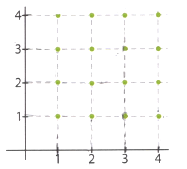
\includegraphics[width=1\linewidth]{6FMA159_imagens/imagem1} \\
			Observe que indicamos os pontos $A = (1; 3)$ e $C = (3; 4)$, e indicamos os pontos $B (2; 2)$ e $D (4; 1)$. Ambas as notações são usuais. \newpage
			\item Representamos a seguir, usando diagramas de Venn, por flechas, o produto cartesiano $\{2, 3, 4\} \times \{2, 4\}$. Assinale as flechas que representam os pares ordenados (2; 4), (3; 2) e (4; 4). \\
			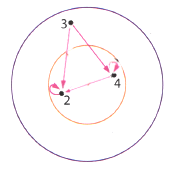
\includegraphics[width=1\linewidth]{6FMA159_imagens/imagem2} \\
			%61 a 63
			\item Dados $A = \{6, 8\}$ e $B = \{1, 3, 5\}$: \\
			\begin{enumerate}[a)]
				\item apresente $A \times B$. \\\\\\\\\\\\\\\\\\\\
				\item represente $A \times B$ usando uma tabela de dupla entrada linha por coluna. \\\\\\\\\\
				\item represente $A \times B$ usando flechas. \\\\\\\\\\\\\\\\\\\\
				\item represente $A \times B$ usando um gráfico cartesiano ortogonal. \\\\\\\\\\\\\\\\\\\\
				\item represente $A \times B$ usando um diagrama de árvore. \newpage
			\end{enumerate}
			\item É apresentado a seguir o gráfico cartesiano ortogonal do produto cartesiano $\{2, 3, 4, 5, 6\}^2$. Localize os seguintes pontos: $A = (3; 2), B = (2; 4), C = (5; 3), D = (4; 4)$ e $E = (6; 6)$. \\
			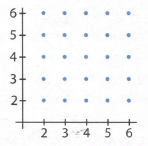
\includegraphics[width=1\linewidth]{6FMA159_imagens/imagem3} \\
			\item Representamos a seguir, usando diagramas de Venn, por flechas, o produto cartesiano $\{2, 3, 4\} \times \{3, 4, 5\}$. Assinale as flechas que representam os pares ordenados (3; 5), (2; 3), (4; 4) e (2; 5). \\
			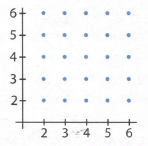
\includegraphics[width=1\linewidth]{6FMA159_imagens/imagem3} \\
		\end{enumerate}
		$~$ \\ $~$ \\ $~$ \\ $~$ \\ $~$ \\ $~$ \\ $~$ \\ $~$ \\ $~$ \\ $~$ \\ $~$ \\ $~$ \\ $~$ \\ $~$ \\ $~$ \\ $~$ \\ $~$ \\ $~$ \\ $~$ \\ $~$ \\ $~$ \\ $~$ \\ $~$ \\ $~$ \\ $~$ \\ $~$ \\ $~$ 
	\end{multicols}
\end{document}